He initialization method was suggested by the \cite{Lachance_2020} paper and has been used in this reseach as well. In order to show the importance of weight initialization choice two experiments have been conducted: in the first on the model predicting nuclei target was trained with the default weight initialization provided by PyTorch and then the initialization was switched to a true He initialization.

\begin{figure}[H]
	\begin{center}
		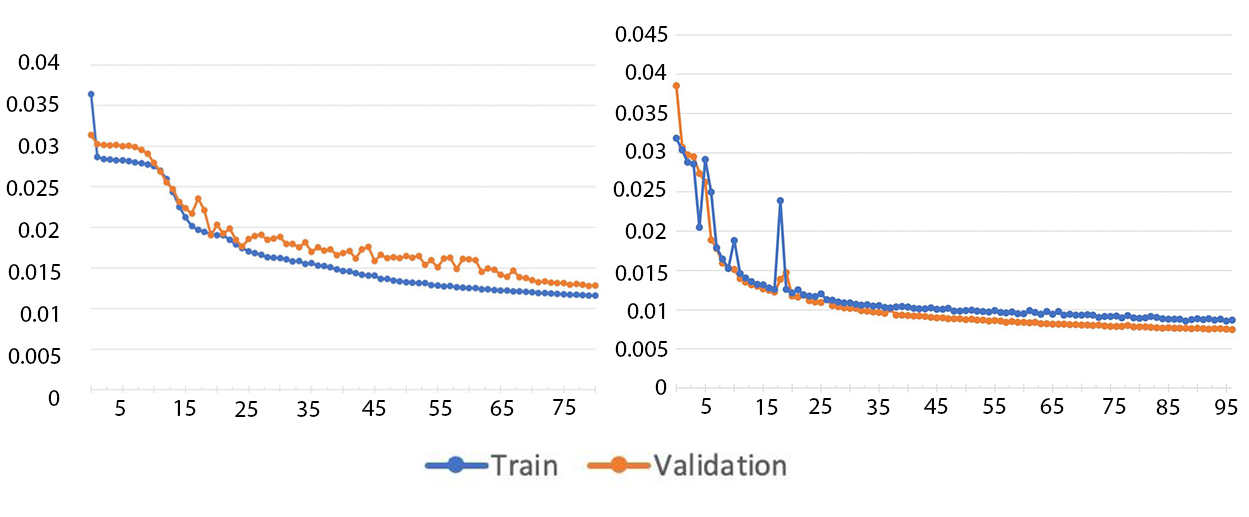
\includegraphics[width=0.8\linewidth]{bilder/nuclei/wi-no-wi.png}
		\caption[Nuclei training without (left) and with (right) custom weight initialization]%
		{Nuclei training without (left) and with (right) custom weight initialization. The stagnation during first few epochs on the left signalizes about the wrong initialization of model's weights. As a result the left model also converges to a higher value.}\label{fig:wi}
	\end{center}
\end{figure}

The results of the experiments are presented in Figure \ref{fig:wi}. As can be seen, the loss in the left plots stagnates during the first few epochs and then begins to converge later. This is a symptom of a wrong initialization of the weights. Even after the convergence begins, the model still has a higher loss than the one on the right (around $0.012$ in comparison to $0.007$). However, the model on the right is not completely perfect as the loss still does not converge at the same speed everywhere. Although this might be not related to the weight initialization but more the to instability of the training in general as there were only few images used for these experiments.
